\documentclass[conference]{IEEEtran}
\IEEEoverridecommandlockouts
% The preceding line is only needed to identify funding in the first footnote. If that is unneeded, please comment it out.
\usepackage{cite}
\usepackage{amsmath,amssymb,amsfonts}
\usepackage{algorithmic}
\usepackage{graphicx}
\usepackage{textcomp}
\usepackage{xcolor}
\def\BibTeX{{\rm B\kern-.05em{\sc i\kern-.025em b}\kern-.08em
    T\kern-.1667em\lower.7ex\hbox{E}\kern-.125emX}}
\begin{document}

\title{Classifying Fruits Using Convolutional Neural Networks\\}

\author{\IEEEauthorblockN{Lewis Lui}
\IEEEauthorblockA{\textit{College of Computer Science} \\
\textit{Cal Poly Pomona}\\
Pomona, US \\
lewislui737@yahoo.com}
\and
\IEEEauthorblockN{Maayan Israel}
\IEEEauthorblockA{\textit{College of Computer Science} \\
\textit{Cal Poly Pomona}\\
Pomona, US \\
zcano@cpp.edu}
\and
\IEEEauthorblockN{Katelyn Mijares}
\IEEEauthorblockA{\textit{College of Computer Science} \\
\textit{Cal Poly Pomona}\\
Pomona, US \\
kmijares@cpp.edu}
\and
\IEEEauthorblockN{Aidan Zimmerman}
\IEEEauthorblockA{\textit{College of Computer Science} \\
\textit{Cal Poly Pomona}\\
Pomona, US \\
azimmerman@cpp.edu}
\and
\IEEEauthorblockN{Sidharth Basam}
\IEEEauthorblockA{\textit{College of Computer Science} \\
\textit{Cal Poly Pomona}\\
Pomona, US \\
Sbasam@cpp.edu}
\and
\IEEEauthorblockN{Ryan}
\IEEEauthorblockA{\textit{College of Computer Science} \\
\textit{Cal Poly Pomona}\\
Pomona, US \\
rtdautel@gmail.com}
\and
\IEEEauthorblockN{Johnny Nguyen}
\IEEEauthorblockA{\textit{College of Computer Science} \\
\textit{Cal Poly Pomona}\\
Pomona, US \\
johnnyn3@cpp.edu}
}

\maketitle

\begin{abstract}
Determining the best architecture is crucial for efficiently classifying images. We compared the accuracy of six architectures, varying the number of dense layers and activation function, training it on the Fruits-360 dataset. The model architecture with the highest accuracy and lowest loss uses the RELU activation function with 3 dense layers. This is because RELU's resistance to the vanishing gradient allows it to take advantage of the additional layers.
\end{abstract}



\section{Introduction}
Determining the best architecture for a given task is crucial for performing that task efficiently. A convolutional neural network (CNN) can have many different types of architectures. Previous works such as Masparudin et al. [6] focused on demonstrating a novel CNN architecture. In this paper, we will compare the performance of existing architectures for academic purposes. To determine which architecture is the best, we built six CNN models with the goal of identifying which architecture best classifies fruits. The CNNs vary along two axes. We will compare the RELU and sigmoid activation functions as well as having one, two, or three dense layers. We will determine what combination results in the best performance.

\section{Dataset Details}

\subsection{Number Of Samples}

We used the Fruits-360 dataset\footnote{https://www.kaggle.com/datasets/moltean/fruits/data}. It contains a total of 52,370 color images of various fruits. These images were collected over time in a controlled laboratory environment using various cameras. All images were unedited and so have varying sizes.

\subsection{Features}
The dataset includes images taken under a wide range of conditions to mimic real-world scenarios. This includes different lighting setups (natural light, shadows, and artificial indoor light), multiple angles and poses, varying numbers of fruits in the frame, and partial occlusions such as hands. All images are in RGB format with 8 bits per channel.

\subsection{Class Distribution}\label{AA}
The dataset includes a range of fruit categories, helping the model learn to recognize both distinct and visually similar fruits. Some fruits have multiple subtypes, such as different kinds of apples, mangoes, and kiwis, allowing for finer classification. The dataset covers the following fruit types and more: apple, banana, carambola, guava, kiwi, mango, orange, peach, pear, persimmon, pineapple, plum, pomegranate, tomatoes, and mulberry.

\subsection{Training/Testing Design}
The dataset was split into three subsets:

Training set: 50.06\% of the data, used to train the model.


Validation set: 25.04\% of the data, used to fine-tune model parameters and prevent overfitting.


Test set: 24.90\% of the data, used to evaluate final model performance.


The splitting ensured that no images from the validation or test sets were used during training, providing an unbiased measure of accuracy.
\subsection{Preprocessing}
The dataset consists of 52,370 RGB images of fruits with various resolutions and sizes. To standardize input across the model and reduce computational complexity, all images were resized to 256×256 pixels. Each pixel value was normalized to the range [0,1][0, 1][0,1] by dividing by 255.0. This normalization step improves training stability and convergence speed.To enhance the model’s ability to generalize to unseen data, data augmentation can be applied using TensorFlow’s Image Data Generator.
\section{Methodology}

\subsection{Experimental Setup}
The CNN models were implemented using TensorFlow 2.16.1 with the tf.keras API. All training and evaluation took place on a node of the NCSA supercomputer cluster equipped with NVIDIA GPUs and 256GB RAM. Models were trained using the Adam optimizer with a learning rate of 0.001, batch size of 32, and for 20 epochs per configuration.

Hyperparameters:
\begin{itemize}
  \item Optimizer: Adam
  \item Loss Function: Categorical Crossentropy
  \item Learning Rate: 0.001
  \item Batch Size: 32
  \item Epochs: 20
\end{itemize}

\subsection{Machine Learning Model}
\begin{enumerate}
    \item One layer of thirty-two 2D convolutions, using RELU and a 3x3 kernel
    \item One 2x2 Max Pooling layer
    \item One flattening layer
    \item A series of dense layers, each with two-hundred fifty six neurons
    \item One final dense layer with the softmax activation function
\end{enumerate}
The models were trained using the entire training and validation set. The variables were the number of dense layers between layer 3 and the final layer and the activation function used in those layers.
\subsection{Model Evaluation}\label{SCM}
To assess the performance of the CNNs, the following metrics were used:

Accuracy: Measures the overall percentage of correctly classified images.


Confusion Matrix: Visualizes how many predictions were correct and where the model made mistakes across all fruit categories.


Precision: The proportion of true positive predictions out of all predicted positives (helps identify how many predicted apples were actually apples, or how mangos are different from oranges, different fruits’ color shading, etc.).


Recall (Sensitivity): The proportion of true positives out of all actual positives (useful for understanding how many actual bananas were correctly classified).


F1-Score: The harmonic mean of precision and recall, useful when dealing with imbalanced classes.

\section{Results}

\begin{table}[h!]
    \centering
    \begin{tabular}{|c|c|c|}
    \hline
          & Sigmoid & RELU\\ \hline
         1& 70.70\% & 99.90\%\\ \hline
         2& 28.02\% & 99.99\%\\ \hline
         3& 18.34\% & 100\%\\ \hline
    \end{tabular}
    \vspace{3pt}
    \caption{Accuracy  based on Activation Function vs Number of Dense Layers}
    \label{tab:my_label}
\end{table}

\begin{table}[h!]
    \centering
    \begin{tabular}{|c|c|c|}
    \hline
          & Sigmoid & RELU\\ \hline
         1& 1.147 & 0.0133\\ \hline
         2& 2.9083 & 0.0049\\ \hline
         3& 3.341 & 0.0038\\ \hline
    \end{tabular}
    \vspace{3pt}
    \caption{Loss based on Activation Function vs Number of Dense Layers}
    \label{tab:my_label}
\end{table}

\begin{table}[h!]
    \centering
    \begin{tabular}{|c|c|c|}
    \hline
          & Sigmoid & RELU\\ \hline
         1& 0.7587 & 0.9999\\ \hline
         2& 0.0380 & 1.0\\ \hline
         3& 0.0039 & 1.0\\ \hline
    \end{tabular}
    \vspace{3pt}
    \caption{Precision based on Activation Function vs Number of Dense Layers}
    \label{tab:my_label}
\end{table}

\begin{table}[h!]
    \centering
    \begin{tabular}{|c|c|c|}
    \hline
          & Sigmoid & RELU\\ \hline
         1& 0.5133 & 0.9996\\ \hline
         2& 0.0786 & 1.0\\ \hline
         3& 0.0212 & 1.0\\ \hline
    \end{tabular}
    \vspace{3pt}
    \caption{ Recall based on Activation Function vs Number of Dense Layers}
    \label{tab:my_label}
\end{table}

\begin{table}[h!]
    \centering
    \begin{tabular}{|c|c|c|}
    \hline
          & Sigmoid & RELU\\ \hline
         1& 1.147 & 0.0133\\ \hline
         2& 2.9083 & 0.0049\\ \hline
         3& 3.341 & 0.0038\\ \hline
    \end{tabular}
    \vspace{3pt}
    \caption{F1 Measure based on Activation Function vs Number of Dense Layers}
    \label{tab:my_label}
\end{table}



\subsection{Analysis/Discussion}
As observed in Table \#1, the CNN that used three dense layers and the RELU activation function performed the best, with a 100\% accuracy.

As observed in Table \#2, the CNNs that used the sigmoid activation function actually had more loss when implemented with more dense layers. In contrast, CNNs that used the RELU activation function actually improved and had less loss as the number of dense layers increased. 

The results clearly show that the RELU (Rectified Linear Unit) activation function dramatically outperformed our sigmoid activations in both accuracy and loss. This is likely due to ReLU's ability to mitigate the vanishing gradient problem, via only saturating in one direction\cite{b7}. The ReLU function outputs 0 for negative inputs and returns the input itself for positive values. This behavior introduces non-linearity into the model, which can be observed graphically as a piecewise linear function with a slope of 0 for negative inputs and a slope of 1 for positive inputs. This in turn is what allows the ReLU activation function to add non-linearity.
As the number of dense layers increases, the RELU-based models continue to improve.
However, in comparison to our ReLU-based models, our sigmoid-based models noticeably degraded as more dense layers were applied, whose output could be interpreted as a probability due to the activation function's nature. This was likely due to vanishing gradients affecting deeper architectures. Because there are more layers, the magnitude of the changes shrinks in the later layers due to the gradient being calculated with more neurons. Updating to differentiate between different classes is ineffective due to the gradient "vanishing" in the upper layers, so the model learns to only predict the most common target class.


Misclassifications were primarily seen in fruits with visually similar appearances For example, in figure 1, 11 quinces are predicted to be apples. This highlights the need for more robust fine-grained visual distinction capabilities in future model improvements. In figures 4-6, you can see how adding more sigmoid layers causes mode collapse. When the architecutre hits three densely connected layers of the sigmoid function, the model predicts that every fruit is an apple. This is caused by the vanishing gradient.

\subsection{Future Work}
\begin{itemize}
  \item Incorporate transfer learning using pre-trained CNNs such as ResNet or MobileNet to reduce training time.
  \item Apply Grad-CAM \footnote{https://github.com/jacobgil/pytorch-grad-cam} to visualize which parts of the image influenced decisions.
  \item Expand the dataset to include more fruits and real-world images from markets to make it more adaptable and resilient to new images. 
  \item Implement lightweight CNN architectures suitable for mobile deployment. This will make CNNs more accessible to a wider audience.
  \item Combine similar class labels (e.g., "apple" and "apple\_") to improve performance. This will help with overfitting.
\end{itemize}
\section{Related Work}
Olimov et al.~\cite{b8} proposed a weight initialization technique based on the ReLU activation function to improve the performance of convolutional neural networks (CNN).

Similarly, Hidenori Ide and Takio Kurita [5] observed in their experiment on the introduction of spare regulation that it led to an improvement in the overall performance of CNNs.

\section{Conclusion}
Our findings show that the combination of the ReLU (Rectified Linear Unit) activation function and three dense layers consistently yields the most accurate and effective CNN architecture for fruit image classification. As shown in our evaluation metrics, this configuration has the highest accuracy of 100\% and the lowest loss of 0.0038. This suggests that deeper architectures with RELU activation are better fitted to extract complex features from varied image data such as the fruit dataset used in our study. With the RELU activation function, we found that increasing the number of dense layers also increased the accuracy of the model. Therefore, we can conclude that the more dense layers we have, the more complex and therefore accurate connections and models were created. 

\begin{thebibliography}{00}

\bibitem{b1} Gorgolewski, C. (2020, February 4). Fruit recognition. Kaggle.
\bibitem{b2} Hongyu, C. Adam Algorithm. URL: https://github.com/keras-team/keras/blob/v3.3.3/keras/src/optimizers/adam.py
\bibitem{b3} 8bitmp3. Convolutional Neural Network. URL: https://github.com/tensorflow/docs/blob/master/site/en/tutorials/images/cnn.ipynb.
\bibitem{b4} Module: Tf.keras  :  tensorflow V2.16.1. TensorFlow. (n.d.). https://www.tensorflow.org/api\_docs/python/tf/keras
\bibitem{b5} Ide, H., \& Kurita, T. (2017). Improvement of learning for CNN with ReLU activation by sparse regularization. 2017 International Joint Conference on Neural Networks (IJCNN). https://doi.org/10.1109/ijcnn.2017.7966185
\bibitem{b6} Masparudin Masparudin, Iskandar Fitri, \& Sumijan Sumijan. (2024). Development of Apple Fruit Classification System using Convolutional Neural Network (CNN) MobileNet Architecture on Android Platform. Sistemasi: Jurnal Sistem Informasi, 13(1), 230–243. https://sistemasi.ftik.unisi.ac.id/index.php/stmsi/article/view/3533/626
\bibitem{b7} Glorot, X., Bordes, A. \&amp; Bengio, Y.. (2011). Deep Sparse Rectifier Neural Networks. \textit{Proceedings of the Fourteenth International Conference on Artificial Intelligence and Statistics}, in \textit{Proceedings of Machine Learning Research} 15:315-323 Available from https://proceedings.mlr.press/v15/glorot11a.html.
\bibitem{b8} Olimov, Bekhzod et al. “Weight Initialization Based‐rectified Linear Unit Activation Function to Improve the Performance of a Convolutional Neural Network Model.” Concurrency and computation 33.22 (2021): n. pag. Web.


\end{thebibliography}
\clearpage
\onecolumn
\begin{figure}[h!]
    \centering
    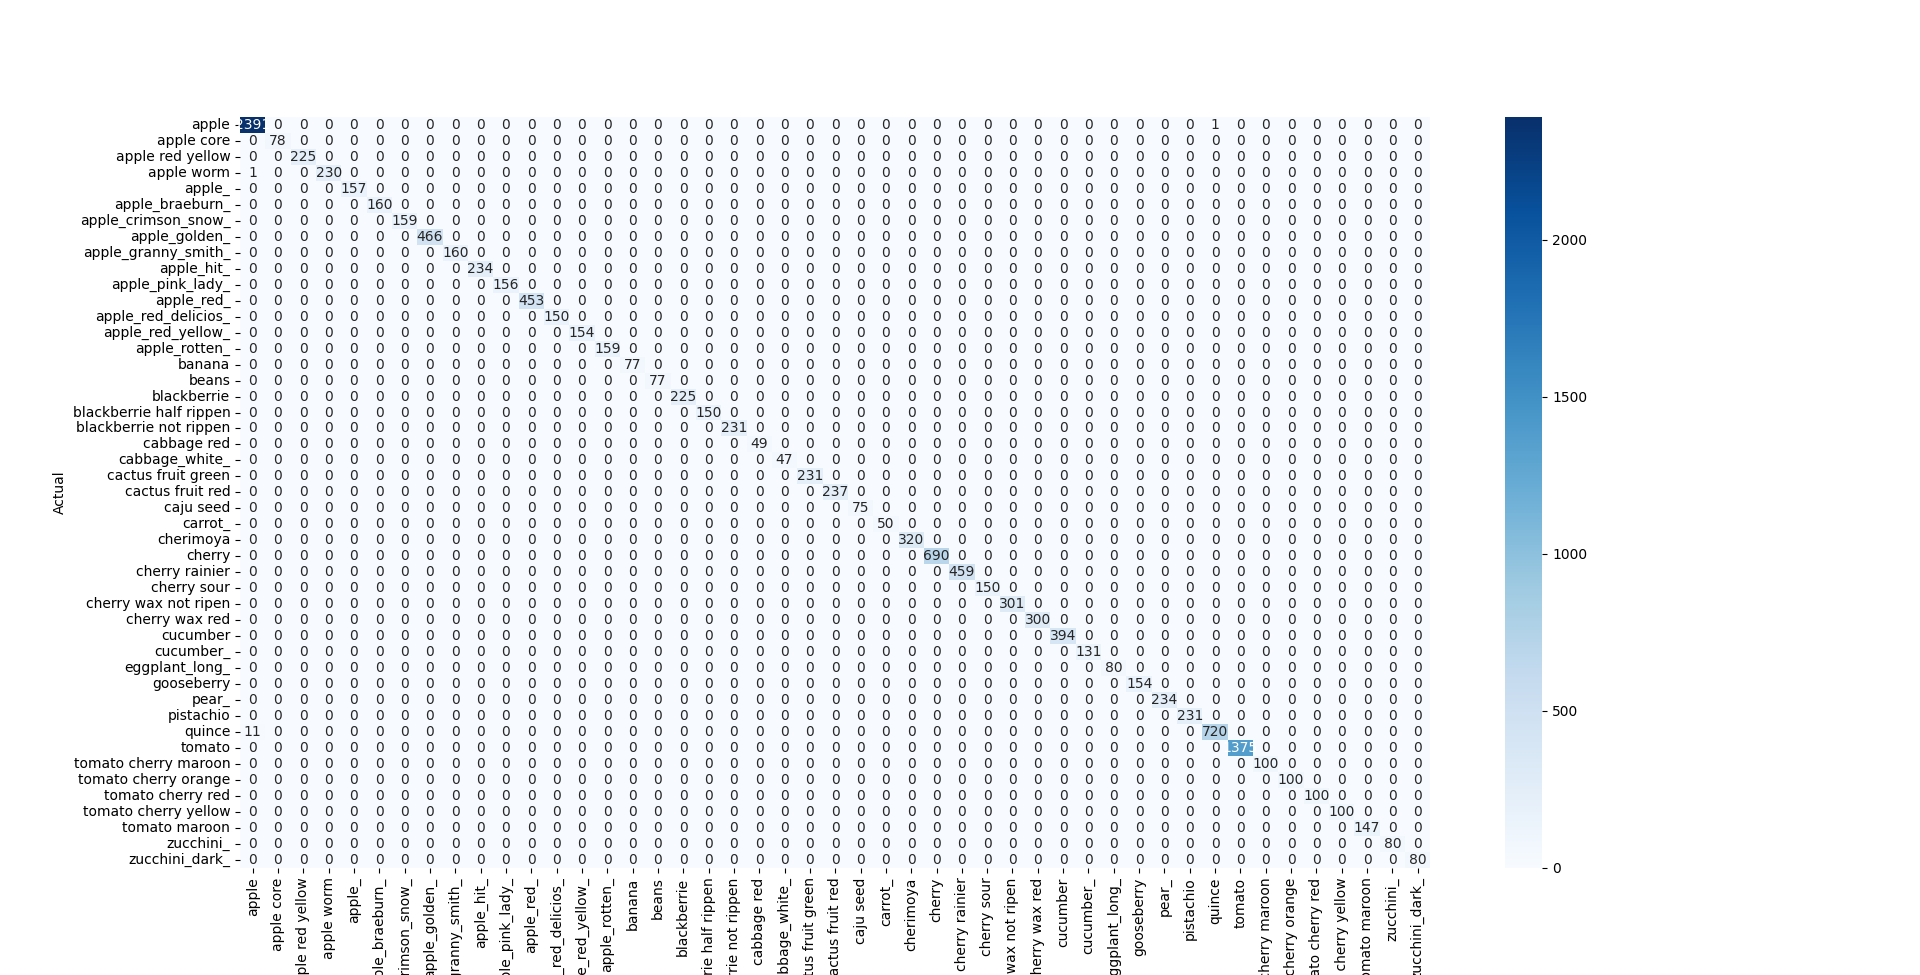
\includegraphics[width=\linewidth]{relu1}
    \caption{Confusion Matrix for RELU1}
\end{figure}

\begin{figure}[h!]
    \centering
    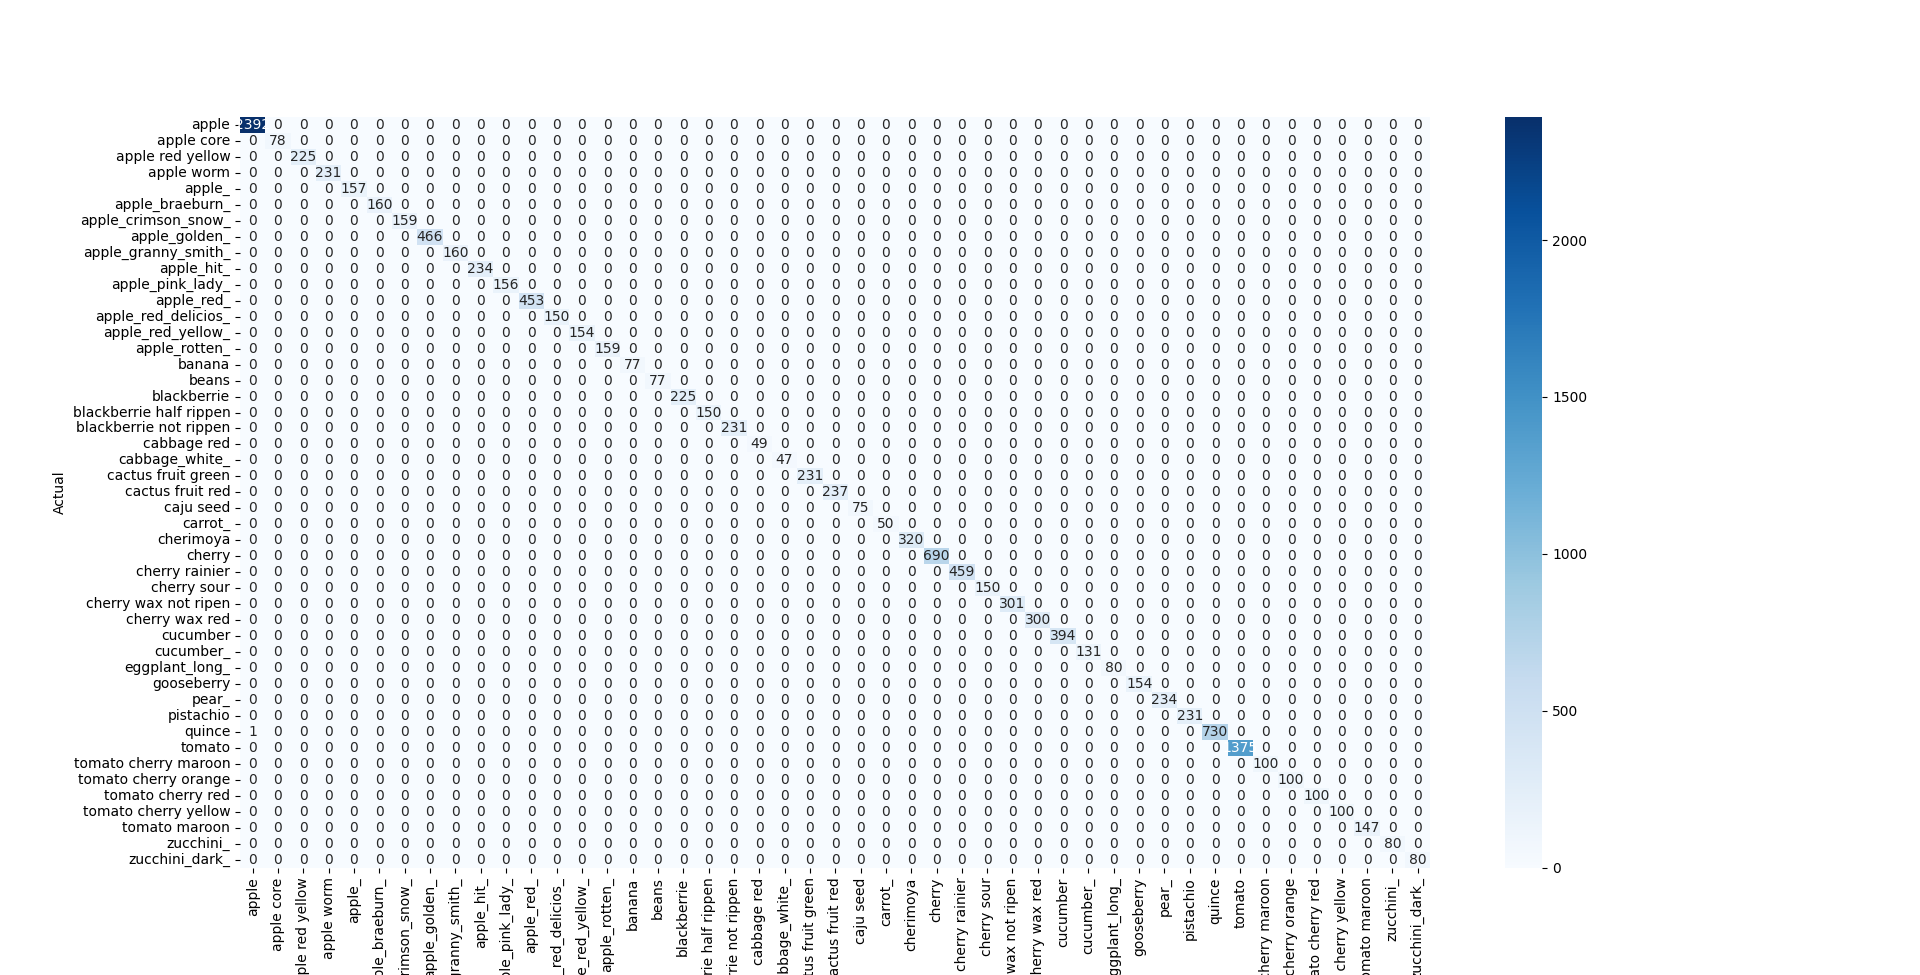
\includegraphics[width=\linewidth]{relu2}
    \caption{Confusion Matrix for RELU2}
\end{figure}

\begin{figure}[h!]
    \centering
    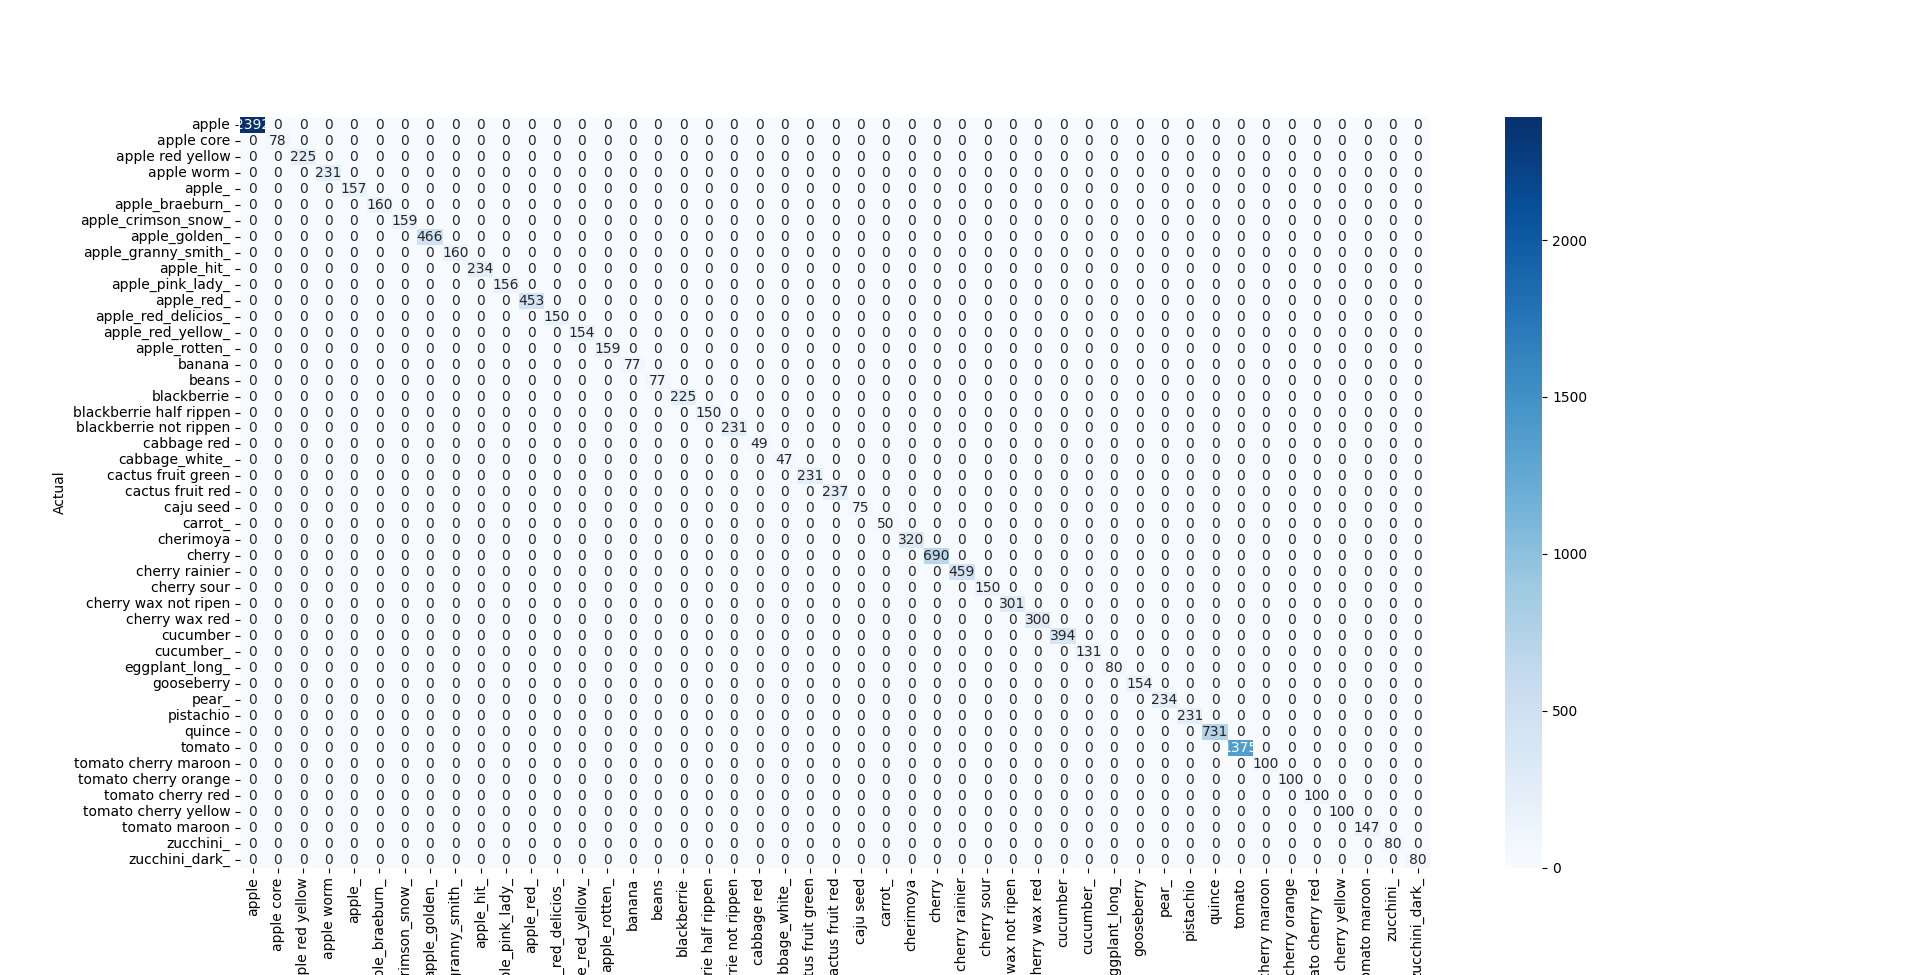
\includegraphics[width=\linewidth]{relu3}
    \caption{Confusion Matrix for RELU3}
\end{figure}

\begin{figure}[h!]
    \centering
    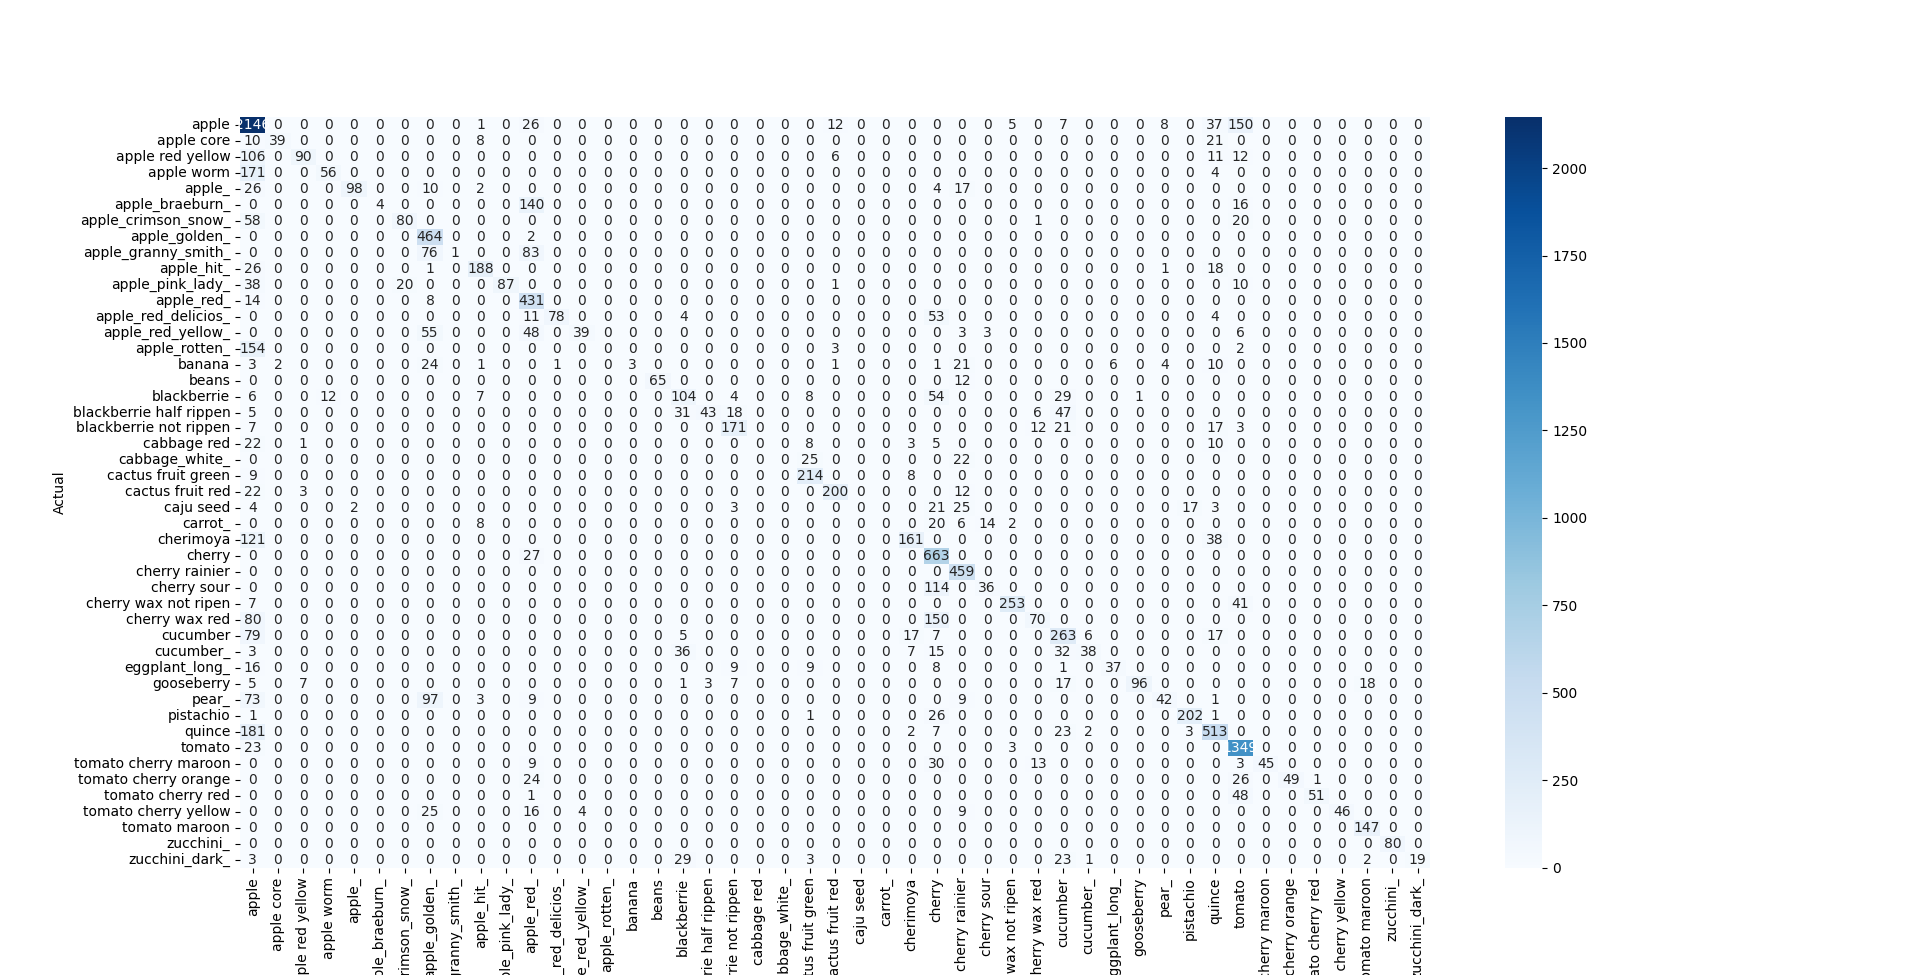
\includegraphics[width=\linewidth]{sigmoid1}
    \caption{Confusion Matrix for Sigmoid1}
\end{figure}

\begin{figure}[h!]
    \centering
    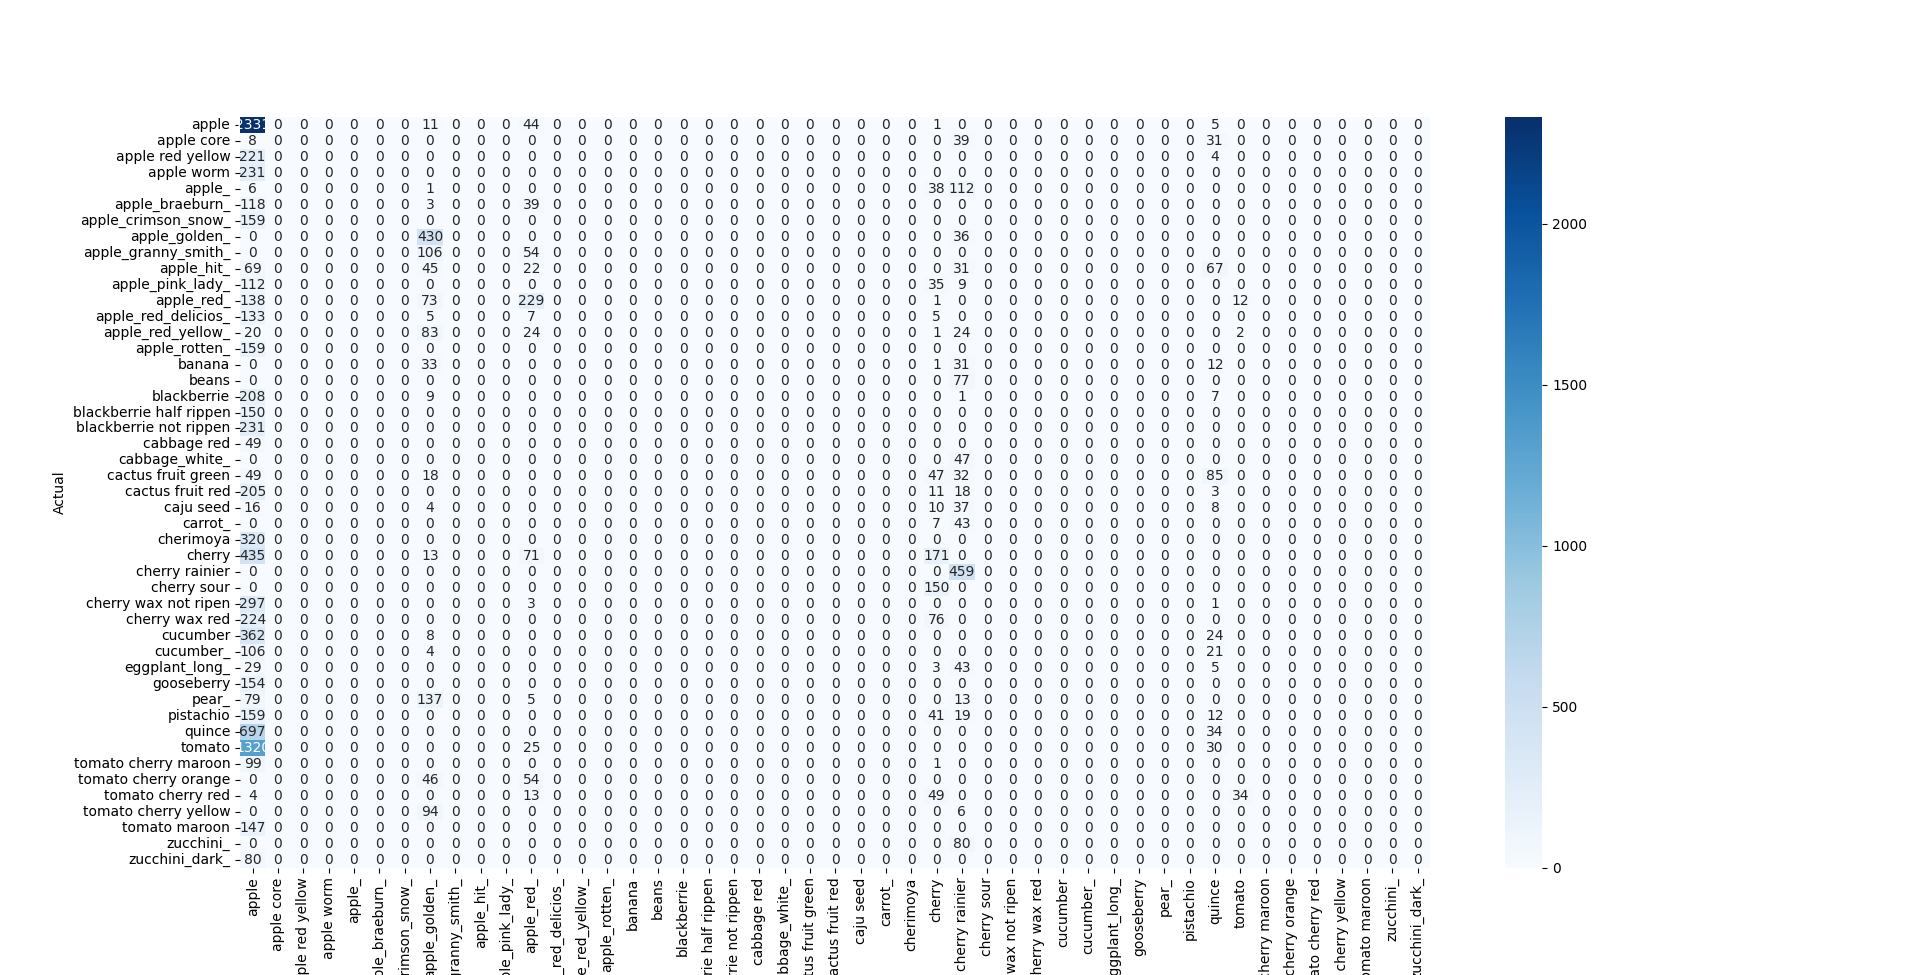
\includegraphics[width=\linewidth]{sigmoid2}
    \caption{Confusion Matrix for Sigmoid2}
\end{figure}

\begin{figure}[h!]
    \centering
    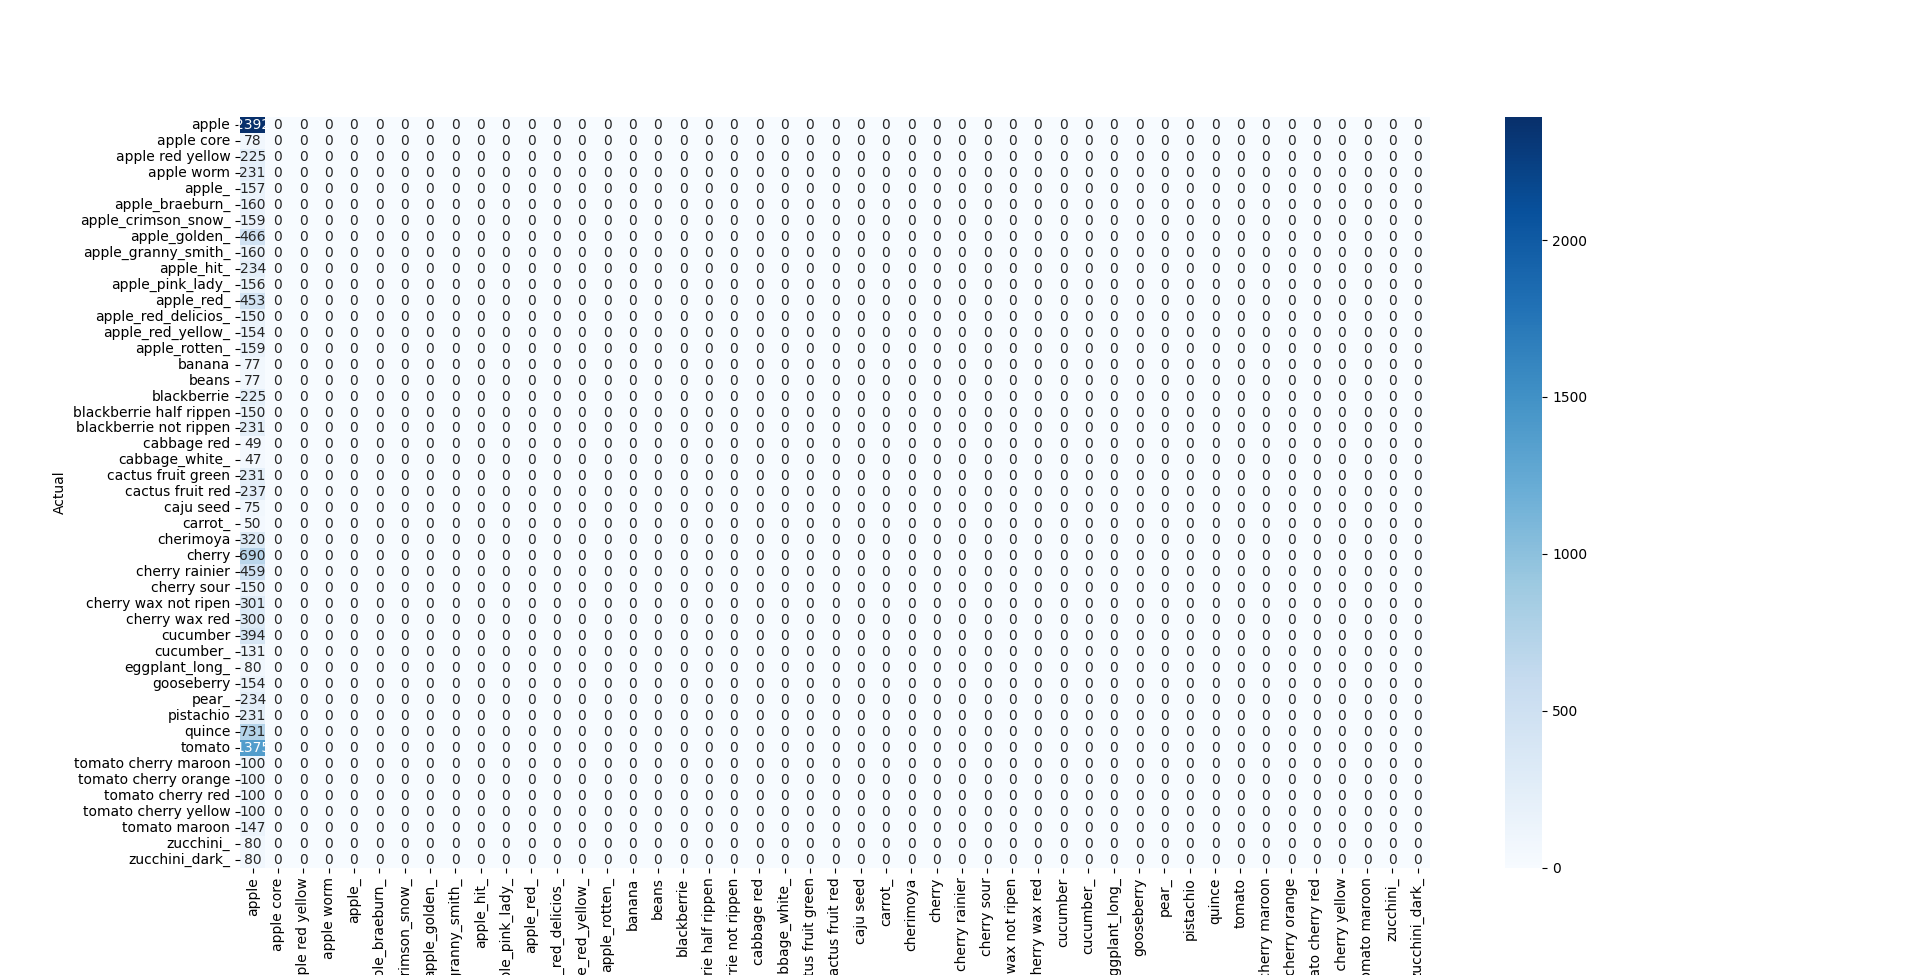
\includegraphics[width=\linewidth]{sigmoid3}
    \caption{Confusion Matrix for Sigmoid3}
\end{figure}
\end{document}